\documentclass[pdftex,a4paper, oneside, openright, 10pt]{article}
\usepackage{newlfont}
\usepackage{colortbl}
\usepackage{ucs}


\definecolor{gray}{rgb}{0.8,0.85,0.85}

\usepackage[utf8x]{inputenc}
\PrerenderUnicode{àèéìòù–}
\usepackage{vmargin}
\usepackage{amssymb}
\usepackage[english]{babel}
\usepackage[breaklinks=true]{hyperref}
\hypersetup{
    %bookmarks=true,         % show bookmarks bar?
    bookmarksopen=false,    % Open up the bookmark tree (Default: false).
    unicode=false,          % non-Latin characters in Acrobat’s bookmarks
    pdftoolbar=true,        % show Acrobat’s toolbar?
    pdfmenubar=true,        % show Acrobat’s menu?
    pdffitwindow=false,     % window fit to page when opened
    pdfstartview={FitH},    % fits the width of the page to the window
    pdfpagemode=UseThumbs,  % Thumbnails are visible
    %pdftitle={},           % title
    pdfauthor={Author},     % author
    %pdfsubject={Audit},                % subject of the document
    pdfcreator={Author},                % creator of the document
    %pdfproducer={\acs{XXX}},           % producer of the document
    %pdfkeywords={XXX, YYY}             % list of keywords
    pdfnewwindow=true,                  % links in new window
    colorlinks=true,                    % false: boxed links; true: colored links
    linkcolor=black,                     % color of internal links
    citecolor=green,                    % color of links to bibliography
    filecolor=magenta,                  % color of file links
    urlcolor=cyan                       % color of external links
}

%\usepackage{titlesec}
\usepackage{minitoc}
%\usepackage{titlesec}

\usepackage{ae}
\usepackage[T1]{fontenc}
\usepackage[printonlyused]{acronym}
\usepackage{graphicx}  % insert [draft] before {...} not to see imgs
\graphicspath{{../images//}}
\usepackage{subfigure}
\usepackage{fancyhdr}
\usepackage{lastpage}
\usepackage{indentfirst}
\usepackage{color}
\usepackage{threeparttable}
\usepackage{longtable}
\usepackage{caption}
\captionsetup{width=.90\textwidth, font={small}, labelfont=bf, format=hang, indention=-45pt}    % to customize the caption
\usepackage{amsmath}
% For analytical index
\usepackage{makeidx}
\makeindex
\usepackage{setspace}
%\usepackage{breakurl}
\usepackage{lscape}

\renewcommand{\rmdefault}{phv} % Arial
\renewcommand{\sfdefault}{phv} % Arial

\singlespacing

\setcounter{secnumdepth}{4}
\setcounter{tocdepth}{4}


%\fancyheadoffset[C]{50pt}
\pagestyle{fancy}

\fancyhead[R,RO]{
\begin{tabular}{l}
Doc \#:\dn\\
Date: {\dt}\\
Page: \thepage~of \pageref{LastPage}
\end{tabular}
$ $\\
}%{\slshape \rightmark}

\fancyhead[CO,C]{
%\bfseries ALMA Project\\
\hspace{-120pt}{\bf\Large \protect\parbox{.4\textwidth}{\textbf{\tit}}}
$ $\\
$ $\\
}%{\slshape \leftmark}

\fancyhead[LO,L]{
%{\bf\Large \tit}

\includegraphics[scale=0.4, angle=0]{almaLogo}
%\fancyfoot[C]{}
}%{\slshape \leftmark}
\renewcommand{\headrulewidth}{1pt}
\setlength{\headheight}{70pt}


\begin{document}
\DeclareGraphicsExtensions{.png, .eps, .jpeg, .giff, .pdf}

% Variable Definition ----------------------------------------------------
\newcommand{\dn}{CORL-64.00.00.00-00XX-A-REP}                % Doc. Number
\newcommand{\dt}{2022-10-18}                                   % Date
%\newcommand{\tit}{\protect\parbox{.4\textwidth}{Single-Dish Continuum \\ Observations at ALMA}}
\newcommand{\tit}{7m-Array Correlation with the 64-Input Correlator}


\newcommand{\preparedBy}
{
Seiji Kameno   &  System Astronomer, Array Performance Group, JAO  & \\
& & \\
Jennifer Donovan Meyer &  CASA Team, NAASC, NRAO & \\
& & \\
Atonio Hales & Array Performance Group Manager, JAO & \\
& &
}

\newcommand{\approvedBy}
{
& & \\
& & \\
& & \\
& &
}

\newcommand{\authorizedBy}
{
& &
}

\newcommand{\changeRecord}{
 A.1     &  {2022-10-20}& All       &  Kameno, Donovan Meyer, Hales &  Initial draft \\
 
}

\newcommand{\ve}{Version}                                        % Version
\newcommand{\st}{Status}                                         % Status
\newcommand{\gr}{\textsuperscript{$\circ$}}
% to insert notes on the text
\newcommand{\mar}[1]{\leavevmode\marginpar{\tiny\raggedright#1\par}}% right note
\newcommand{\nota}[1]{%
  \marginpar[{\raggedleft\small\sffamily #1\\}]{%
    {\raggedright\footnotesize\sffamily #1\\}}}

% Cover Page ----------------------------------------------------
\thispagestyle{empty}
\setlength{\voffset}{-70pt}
\setlength{\oddsidemargin}{70pt}
\vspace*{-3cm}

\includegraphics[scale=0.45, angle=0]{ima-000.png}
\hskip 1.0 cm
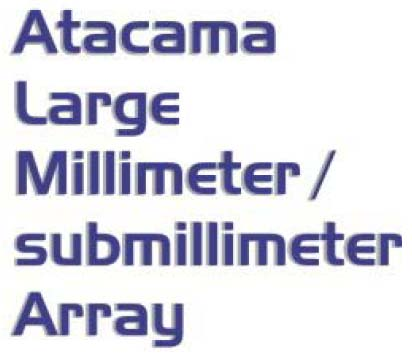
\includegraphics[scale=0.35, angle=0]{ima-001.png}



\begin{center}
    \vskip 2 cm
    {\Huge{\textbf{\tit}}}\\   %\newcommand{\tit}{\protect\parbox{.4\textwidth}{Single-Dish Continuum \\ Observations at ALMA}}

    \vskip 2 cm
\Large {\dn}\\
%Version: {\ve}\footnote{Printed versions of this document are For Reference Only. The latest released electronic version is located in the \acs{ALMA} \ac{EDM} system accessible through the internet at: \href{http://edm.alma.cl}{http://edm.alma.cl}}
%\\
%Status: {\st}\\
\vskip 2 cm
{\dt}\\
\vskip 2 cm



\begin{table}[htbp]
\centerline{
\begin{tabular}{|p{5cm}|p{5cm}|p{5cm}|}
  \hline
  % after \\: \hline or \cline{col1-col2} \cline{col3-col4} ...
  \rowcolor{gray} {\bf Prepared By:}                    & {\bf Organization Role} & {\bf Date  and Signature}    \\\hline
                                        &  &  \\
                                        &  &  \\
  \preparedBy                         \\
                                        &  &  \\
                                        &  &  \\\hline
  \rowcolor{gray} {\bf Approved By:}                    & {\bf Organization Role} &{\bf  Date and Signature } \\\hline
                                        &  &  \\
                                        &  &  \\
  \approvedBy                                  \\
                                        &  &  \\
                                        &  &  \\\hline
  \rowcolor{gray} {\bf Authorized By:}                  & {\bf Organization Role} &{\bf  Date and Signature } \\\hline
                                        &  &  \\
                                        &  &  \\
  \authorizedBy                                  \\
                                        &  &  \\
                                        &  &  \\\hline
\end{tabular}}
\end{table}
\end{center}


\setlength{\voffset}{-90pt}
\setlength{\oddsidemargin}{90pt}
\setlength{\textheight}{600pt}
\clearpage


\section*{Change Record}
\thispagestyle{fancy}
%\addcontentsline{toc}{chapter}{Change Record}
\begin{table}[htbp]
\centerline{
\begin{tabular}{|c|c|c|c|l|}
  \hline
  % after \\: \hline or \cline{col1-col2} \cline{col3-col4} ...
 \rowcolor{gray} Version   &   Date  &  Affected Section(s)    &  Author &  Reason, Initiation, Remarks\\\hline
  \changeRecord
\hline
\end{tabular}}

\end{table}

%\frenchspacing
%\dominitoc

%\thispagestyle{fancy}
%\addcontentsline{toc}{chapter}{\contentsname}
%\begingroup
%\let\clearpage\relax
\tableofcontents
%\thispagestyle{fancy}
%\endgroup


\begingroup
\let\clearpage\relax
\listoffigures{}
\thispagestyle{fancy}
\endgroup


%\addcontentsline{toc}{chapter}{\listfigurename}

%\listoftables
%\thispagestyle{fancy}

\clearpage

%\addcontentsline{toc}{chapter}{\listtablename}

%\clearpage
\chapter*{Change Record}
\thispagestyle{fancy}
\addcontentsline{toc}{chapter}{Change Record}
\begin{table}[htbp]
\centerline{
\begin{tabular}{|c|c|c|l|}
  \hline\hline
  % after \\: \hline or \cline{col1-col2} \cline{col3-col4} ...
  Version   &   Date  &  Affected Section(s)    &   Reason, Initiation, Remarks\\\hline\hline
  A     &  {\dt}  & All     & First Issue   \\\hline
        &         &         &               \\\hline\hline
\end{tabular}}
\caption{Change Record Table}
\end{table}

  % Change Request insertion
%\clearpage
\chapter*{Acronyms}
\thispagestyle{fancy}
\addcontentsline{toc}{chapter}{Acronyms}
\markboth{ACRONYMS}{ACRONYMS}

\begin{acronym}
% A---------------------------------------------------------------
\acro{ACRV}{Acceptance Review}
\acro{ADE}{\acs{ALMA} Department of Engineering}
\acro{ADPK}{Acceptance Data Package}
\acro{AEM}{ALMA European Consortium}
\acro{AI}{Action Item}
\acro{AIPC}{Antenna Inspection Point in Chile}
\acro{AIPT}{Antenna Integrated Product Team}
\acro{AIV}{Assembly Integration Verification}
\acro{ALMA}{Atacama Large Millimeter/submillimeter Array}
\acro{AOB}{Any Other Business}
\acro{ATU}{Air Treatment Unit}

% B---------------------------------------------------------------

% C---------------------------------------------------------------
\acro{CAD}{Computer Aided Design}
\acro{CAN}{Controller Area Network}
\acro{CIDL}{Configuration Item Data List}
\acro{CRE}{Change Request}
% D---------------------------------------------------------------
\acro{DC}{Direct Current}
\acro{DoC}{Declaration of Conformity}
\acro{DPK}{Data Package}
\acro{DSP}{Digital Signal Processor}
% E---------------------------------------------------------------
\acro{EIE}{European Industrial Engineering}
\acro{EDM}{Engineering Data Management}
\acro{ESO}{European Southern Observatory}
\acro{EU}{European}
% F---------------------------------------------------------------
\acro{FEA}{Finite Element Analysis}
%\acro{FMECA}{Failure Mode, Effects and Criticality Analysis}
% G---------------------------------------------------------------
%
% H---------------------------------------------------------------
\acro{HVAC}{Heating, Ventilating and Air Conditioning}
% I---------------------------------------------------------------
\acro{IPT}{Integrated Product Team}
% K---------------------------------------------------------------

% L---------------------------------------------------------------
\acro{LCD}{Liquid Crystal Display}
% M---------------------------------------------------------------
\acro{MT-A}{MT-Aerospace}
\acro{MoM}{Minutes of Meeting}
% N---------------------------------------------------------------
\acro{NA}{Not Available}
\acro{NAm}{North American}
\acro{NAp}{Not Applicable}
\acro{NAOJ}{National Astronomical Observatory of Japan}
\acro{NCR}{Non Conformance Report}
\acro{NRAO}{National Radio Astronomy Observatory}
% O---------------------------------------------------------------
\acro{OSF}{Operations Support Facility}
% P---------------------------------------------------------------
\acro{PA}{Product Assurance}
\acro{PAI}{Preliminary Acceptance in House}
\acro{PAS}{Preliminary Acceptance on Site}
% Q---------------------------------------------------------------
\acro{QA}{Quality Assurance}
% R---------------------------------------------------------------
\acro{RFW}{Request for Waiver}
\acro{RID}{Review Item Discrepancy}
\acro{RP}{Review Panel}
% S---------------------------------------------------------------
\acro{SE}{Systems Engineering}
\acro{SEF}{Site Erection Facility}
% T---------------------------------------------------------------
\acro{TBA}{To Be Added}
\acro{TBD}{To Be Defined}
\acro{TRR}{Test Readiness Review}
\acro{TAS}{Thales Alenia Space}
% U---------------------------------------------------------------

% V---------------------------------------------------------------

% W---------------------------------------------------------------
\acro{WI}{Workmanship Inspection}
\acro{wrt}{with respect to}
% J---------------------------------------------------------------
\acro{JAO}{Joint \acs{ALMA} Office}
% Z---------------------------------------------------------------
\end{acronym}   % Acronyms insertion
%\clearpage
\chapter*{Verb Convention}
\thispagestyle{fancy}
\addcontentsline{toc}{chapter}{Verb Convention}
\markboth{VERB CONVENTION}{VERB CONVENTION}

The following verb convention shall apply in this document:
\begin{itemize}
  \item The word \emph{shall} in the text is used to indicate a mandatory item;
  \item The word \emph{should} in the text is used to indicate a desirable but not mandatory item;
  \item The word \emph{will} in the text is used to indicate an expression of future intent but not a mandatory item;
  \item The word \emph{must} in the text expresses an assumption, the fulfillment of which is outside the scope of this document;
  \item The word \emph{may} in the text expresses a permissible practice or action. It does not express a requirement;
  \item The use of the present tense (e.g. is, are) indicates that the associated statement is explanatory material provided in support of the document.
\end{itemize}

    % Verbs convention


%---------------------------BODY START---------------------------------
%\input{../body/body.tex}
\clearpage
%\section{Abstract}
%This document is a comprehensive report about the status of single-dish continuum observations with ALMA...BlaBla...

%\clearpage
\section{Introduction}
\thispagestyle{fancy}


\subsection{Purpose}
This document reports verifications of correlation processing for the 7m-array observations using the 64-input correlator (also known as BLC).

Currently, as of Cycle 9, the ACA correlator (ACAC) is used for the Morita array (the 7m array and the TP array) processing. Since Cycle 10, the ACA spectrometer (ACASPEC) is planned to take over the spectroscopy processing for the TP array and the ACAC will dedicates to 7m-array correlation.
The BLC is also capable to perform subarray correlations for the 12m array and the 7m array, in parallel, when the ACAC is out of service. This 7m-array correlation using the BLC is a contingency plan for troubles or future decommission plan of the ACAC.

To validate the BLC correlation of the 7m array for science operations, we have carried out commissioning science verification (CSV) activities. Here we present the results of the CSV.


%\begin{tabular}{|p{1.0cm}|p{6.5cm}|p{6.8cm}|}
\subsection{Applicable documents}
The following documents are part of this document to the extent specified herein.
If not explicitly stated otherwise, the latest issue of the document is valid.\\
\begin{tabular}{|p{1.2cm} | p{8.5cm} | p{4.5cm}|}
\hline
\rowcolor{gray} \bf Appl. & \bf Document Title &\bf Doc.\\
\hline
$[$AD01$]$ &ACA Spectrometer Technical Specifications and Requirements   					& \href{http://edm.alma.cl/forums/alma/dispatch.cgi/iptdocscorr/showFile/101189/d20210529211811/Yes/2021-04-09-ALMA-64.00.00.00-005-C-SPE-ACA_Spectrometer+Technical+Specifications.pdf}{ALMA-64.00.00.00-0005-B-SPE} \\
$[$AD02$]$ &ACA Spectrometer Assembly, Transportation, Integration and Verification Plan  	& \href{http://edm.alma.cl/forums/alma/dispatch.cgi/iptdocscorr/docProfile/101235/d20191209084810}{CORL-64.00.00.00-0022-A-PLA} \\
$[$AD03$]$ &ACA Spectrometer Subsystem Design Description   								& \href{http://edm.alma.cl/forums/alma/dispatch.cgi/iptdocscorr/docProfile/101230/d20200610070519}{CORL-64.00.00.00-0008-A-DSN} \\
$[$AD04$]$ &Report on Dynamic Range, Nonlinearity Correction and Delay Correction Implemented into the ACA Spectrometer  & \href{http://edm.alma.cl/forums/alma/dispatch.cgi/iptdocscorr/docProfile/101273/d20200825044738/No}{CORL-64.00.00.00-0028-A-REP} \\
$[$AD05$]$ &ACA spectrometer Commissioning and Science Verification Plan  & \href{http://edm.alma.cl/forums/alma/dispatch.cgi/iptdocscorr/docProfile/101273/d20200825044738/No}{CORL-64.00.00.00-0028-A-REP} \\
\hline
\end{tabular}

\subsection{Reference documents}
The following documents contain additional information and can be referenced in this document.\\
\begin{tabular}{|p{1.2cm} | p{8.5cm} | p{4.5cm}|}
\hline
\rowcolor{gray} \bf Ref. & \bf Document Title &\bf Doc.\\
\hline
$[$RD01$]$ & ALMA System Technical Requirement &  \href{}{ALMA-80.04.00.00-005-C-SPE} \\
\hline
\end{tabular}

%\subsection{Acronyms}
%For a complete set of acronyms and abbreviations used in the ALMA project, please go to the Acronym Finder [AD01].

\clearpage


\section{CSV test items}

\subsection{Specifications and requirements}\label{sec:spec}
Table \ref{tab:label}  shows the technical specifications and requirements verified through the CSV activities with corresponding CSV-tickets. The full descriptions of technical specifications and requirements of the ACA spectrometer shall be referred to [AD01].  In addition to them, we added test items that are more similar to the actual science operations such as end-to-end like testing.

\begin{longtable}{|p{3cm}|p{2cm}|p{6cm}|p{2cm}|}
%\begin{tabular}
\caption{Summary of specifications and requirements for the ACA spectrometer\label{tab:label}}\\ \hline
Parameter                         & Req. No.                                     & Value                                                                                                                                                                                                                                        & CSV ticket                                                 \\ \hline 
\endfirsthead
\hline
Parameter                         & Req. No.                                     & Value                                                                                                                                                                                                                                        & CSV ticket                                                 \\ \hline 
\endhead
IF bandwidth                      & CORL-64.00.00.00-00220-00/R                  & 4 baseband pairs of 2 (polarizations) x 2 GHz (=16 GHz) bandwidth per antenna.                                                                                                                                                               & CSV-3771                                                   \\ \hline 
Spectral resolution               & CORL-64.00.00.00-00230-00/R                  & all the spectral resolutions offered in the observation modes in Table 1-7 of {[}AD01{]}.                                                                                                                                                    & CSV-3771                                                            \\ \hline 
Spectral windows                  & CORL-64.00.00.00-00230-00/R                  & The ACA Spectrometer (as the ACA Correlator) should support the capability to process 64 spectral windows per baseband pair for the future.                                                                                                                                                                                             & CSV-3771                                                            \\ \hline 
Minimum integration time          & CORL-64.00.00.00-00240-00/R                  &     16 ms for auto-only TDM, 32 ms for auto-only FDM, and 96 ms for cross TDM                                                                                                                                                                                                                                         & CSV-3778                                                           \\ \hline
Spectral Dynamic range            & CORL-64.00.00.00-00241-00/R                  & 20000:1 as the ratio of the peak spectral line amplitude to the RMS noise in the spectrum                                                                                                                                                    & CSV-3772                                                           \\ \hline
Spectrometer Products             & CORL-64.00.00.00-00250-00/R                  & XiXi* or YiYi* for single polarization, XiXi* and YiYi* for dual polarization, and XiXi*, YiYi*, XiYi* and YiXi* for full polarization per baseband pair per antenna. XiXj*, YiYj*, XiYj*, YiXj* for only TDMs for calibration observations. & CSV-3771, 3777                                               \\ \hline
Number of antennas                &                                              & up to 4 antennas                                                                                                                                                                                                                                   & CSV-3771                                                            \\ \hline
Number of correlations            &                                              & XX, YY, XY, YX both for auto-correlations and cross-correlations.                                                                                                                                                                            & CSV-3771                                                 \\ \hline
Quantization levels of input data &                                              & 3-bits                                                                                                                                                                                                                                       & All input data should be 3-bits                             \\ \hline
Maximum output data rates         &                                              & The maximum output data rate shall not exceed 17 MB/sec.                                                                                                                                                                                     & CSV-3778                                                           \\ \hline
Sensitivity Loss				  & CORL-64.00.00.00-00305-00/A					 & \textless{}2.1\%. The sensitivity loss of FFT with 5\% overlapped data is less than 2.1\%, which is shown in Sect. 5.4 of {[}AD01{]}.                                                                                         				& Discussion can be found at CSV-3482.				 		  \\ \hline
Delay correction				  &	CORL-64.00.00.00-00308-00/A					 & The sensitivity loss of the ACA Spectrometer due to imperfect delay correction should be smaller than 1\%\footnote{The delay correction with 1 ms resolution will be implemented to achieve this specification at the 16 km baseline. See {[}AD04{]} for the details.}.  & CSV-3756								  \\ \hline
Output data format                & CORL-64.00.00.00-00310-00/R,T                & BDF                                                                                                                                                                                                                                          & all                                                         \\ \hline
Correlator / Spectrometer modes   & CORL-64.00.00.00-00360-00/R                  & autocorrelation and cross correlation (calibration purpose)                                                                                                                                                                                  & CSV-3725, 3770                                                  \\ \hline
Channel-averaging factors         & CORL-64.00.00.00-00370-00/R                  & 2, 4, 8, 16, 32, 64                                                                                                                                                                                                                          & CSV-3771                                                           \\ \hline
Frequency profile  synthesis      & CORL-64.00.00.00-00370-00/A,R                & An option to synthesize the frequency response profile of the 64-input Correlator with a window function is implemented                                                                                                                      & CSV-3774                                                            \\ \hline
Linearity                         & CORL-64.00.00.00-00320-00/R,T                & A total power measurement based on 3-bit digitized signal with nonlinearity correction shall have less than 1\% error relative to the measurement of an analogue power meter over a dynamic range of 10 dB                                   & CSV-3775                                                        \\ \hline
Stability                         & \#261 of {[}RD01{]}                          &  ASD < 1.0* 10-3 on time scales of 0.05 to 100 seconds\footnote{In the original CSV plan ({[}RD05{]}), \#263 of {[}RD01{]} was refereed as the specification of the stability, but it is for the continuum TP observations, which is still not offered by ALMA. \#261 of {[}RD01{]} is more appropriate as the specification for emission line TP observations and shall be verified in the ACASPEC CSV.} & CSV-3757                                                           \\ \hline
Spurious signals                  & \#295.2 of {[}RD01{]}                        & to be suppressed down to 1/3 with respect to the standard deviation (SD) of a 16-hour integrated spectrum with 1-sec on–off cycles and 1-MHz of the spectral resolution.                                                                     & CSV-3727                                                           \\ \hline 
End-to-end test                   &                                              &                                                                                                                                                                                                                                              & CSV-3776                                                           \\ \hline
%\end{tabular}
\end{longtable}

The 90 degrees Walsh switching and the LO offset are not supported by the ACA spectrometer. The 180 degrees Walsh switching is supported by the TP array \footnote{The 180 deg Walsh switching will be inserted in the 1st LO and will be removed by sign reversal in the DTX Formatter. Thus for observations with the 180 deg Walsh switching, the ACA Spectrometer will do nothing special to perform the function.}. 

\newpage
\subsection{CSV tickets}

The ACASPEC CSV activity has been traced by the parent CSV ticket (\href{https://jira.alma.cl/browse/CSV-3724}{CSV-3724}: Commissioning of ACA Spectrometer). 
This parent ticket consists of the following 14 major sub-task tickets to cover the verification of the specifications listed in Section \ref{sec:spec}.  

\begin{enumerate}
\item \href{https://jira.alma.cl/browse/CSV-3724}{CSV-3725} ACASPEC: Calibration executions with manual scripts
\item \href{https://jira.alma.cl/browse/CSV-3725}{CSV-3726} ACASPEC: Line detection using a manual script	
%\item \href{https://jira.alma.cl/browse/CSV-3727}{CSV-3727} ACASPEC: Spurious signal survey	
%\item \href{https://jira.alma.cl/browse/CSV-3755}{CSV-3755} ACASPEC: Linearity test using manual scripts	
\item \href{https://jira.alma.cl/browse/CSV-3756}{CSV-3756} ACASPEC: Delay Correction	
\item \href{https://jira.alma.cl/browse/CSV-3757}{CSV-3757} ACASPEC: Stability of auto-correlation data	
\item \href{https://jira.alma.cl/browse/CSV-3761}{CSV-3761} ACASPEC: Initial test of SB	
\item \href{https://jira.alma.cl/browse/CSV-3770}{CSV-3770} ACASPEC: Calibration executions with SBs	
\item \href{https://jira.alma.cl/browse/CSV-3771}{CSV-3771} ACASPEC: Line detection with SBs	
\item \href{https://jira.alma.cl/browse/CSV-3772}{CSV-3772} ACASPEC: Spectral dynamic range	
\item \href{https://jira.alma.cl/browse/CSV-3773}{CSV-3773} ACASPEC: Jy/K factor	
\item \href{https://jira.alma.cl/browse/CSV-3774}{CSV-3774} ACASPEC: Frequency profile synthesis	
\item \href{https://jira.alma.cl/browse/CSV-3775}{CSV-3775} ACASPEC: Linearity test using SBs	
\item \href{https://jira.alma.cl/browse/CSV-3776}{CSV-3776} ACASPEC: OTF mapping and E2E-like testing	
\item \href{https://jira.alma.cl/browse/CSV-3777}{CSV-3777} ACASPEC: Polarization products	
\item \href{https://jira.alma.cl/browse/CSV-3778}{CSV-3778} ACASPEC: Minimum integration time and Maximum data rate	
%\item \href{https://jira.alma.cl/browse/CSV-3779}{CSV-3779} ACASPEC: TP Spectral Scan
\end{enumerate}


\subsection{CSV activity}

We performed the CSV activity of the ACASPEC in the following periods based on coordination with DSO and the ACASPEC engineering team. We used the Cycle 8 online environment, so that science operations on the 12m and 7m arrays can continue in parallel with the CSV. 
\begin{itemize}
\item \textbf{Initial test after the AIV: 2022 Feb., from OSF}
\item \textbf{CSV Phase 1: 2022-04-20 -- 22, from SCO}
\item \textbf{CSV Phase 2: 2022-06-14 -- 20, from OSF}
\item \textbf{Supplemental CSV: 2022-08-03 -- 04, Remote}
\end{itemize}
The detailed log of executions is available at:\\
\url{https://docs.google.com/spreadsheets/d/1DP73n6_Snm7PqS0fzzfuH2hidyVEI3UbF8lZSXwDKfo/edit?usp=sharing}  

\newpage
\section{CSV resuts}\label{sec:result}
In this section, we describe the resuls of the CSV observation for each CSV ticket. 

\subsection{Calibration executions with manual scripts (CSV-3725)}
First, we tested the array creation of the Total Power array with the ACASPEC. Both manual and dynamic arrays have been created without problem by the array operator. TP array with the ACASPEC appears as ``ArrayXX-TPS'' in the OMC, the Array Summary, and the Shiftlog tool (SLT). Currently ``TPS array'' does not associate with the TP array family, and all the executions are logged as manual executions (MMEX entries in the SLT). This issue will be fixed at ICT-20158 (see Section \ref{sec: updates}).   

To verify the spectrometer products of cross-correlations, we tested calibration observations using manual scripts such as DelayCal (DelayCal.py) and Focus (InterferometricFocus.py). These scripts were successfully executed from the STE consoles in the control room. 

In the early stages, due to the missing correction of the ACA specific delays (PRTSPR-57618), large delay offsets remain in the cross-correlation data, and no fringes were detected for continuum sources. There were phase jumps (PRTSPR-57385 and PRTSPR-58253) due to bugs in the delay correction in the ACASPEC software. During this test, we also found initial issues such as the malformed BDF header (PRTSPR-57169 and PRTSPR-57171) and incorrect SpW names (PRTSPR-56540, an issue in CONTROL), which prevent TelCal from receiving the data from the ACASPEC. 

After fixing all these issues at ICT-20865 (and SCCB-1233), ICT-20467, ICT-20533, and by updates on ASM, we detected fringes toward standard ALMA calibrator sources correctly without phase jumps, as shown in Figure \ref{fig:DelayCal_listobs}, \ref{fig:DelayCal_freq}, and \ref{fig:DelayCal_time}, and we confirmed the delay correction works as designed. However, some Frequency-Phase plots show slopes that correspond to $\sim$ 0.25 ns at most. We will discuss this in Section 3.5. We also confirmed that TelCal calculates the Delay offset and OuickLook shows the result. The detailed results for the performance of calibration observations will be presented in Section \ref{sec:cal_SB}. DelayCal with the 180-degree Walsh switching option does not show problems. 

\begin{figure}[htbp]
     \centering
    \includegraphics[keepaspectratio, width=120mm]{images/listobs_Xb3f.png}
     \caption{Example of the listobs result for DelayCal with the ACASPEC that shows the expected scan and spw information after fixing initial issues.}
     \label{fig:DelayCal_listobs}
\end{figure}

\begin{figure}[htbp]
     \centering
    \includegraphics[keepaspectratio, width=150mm]{images/PS_uid___A002_Xfa622c_X232e_Scan1_SPW1-1.png}
     \caption{Example of the DelayCal result (EB UID: uid://A002/Xfa622c/X232e). Frequency-Amplitude/Phase plots for each baseline. Blue and green lines show the amplitude or phase of XX and YY polarizations, respectively.}
     \label{fig:DelayCal_freq}
\end{figure}

\begin{figure}[htbp]
     \centering
    \includegraphics[keepaspectratio, width=140mm]{images/X232e_time-amp_phase.pdf}
     \caption{Example of the DelayCal result (EB UID: uid://A002/Xfa622c/X232e). Time-Amplitude (top)/Phase (bottom) plots for each baseline. Pink and black points show the amplitude or phase of XX and YY polarizations, respectively.}
     \label{fig:DelayCal_time}
\end{figure}

\newpage

\subsection{Line detection using a manual script  (CSV-3776)}
The auto-correlation product of the ACA Spectrometer has been verified by the Total Power observations in the SiO($J$=2--1) maser line at 86.243 GHz and CO($J$=1--0) line at 115.235 GHz using DelayCal and ObsCalOffPointCheck.py. The first light has been arhicved on 2022-02-22 (Figure \ref{fig:Firstlight}). 

There was an issue in the Frequency labeling in the FDM mode (PRTSPR-56002) during AIV in February, and this bug was fixed at ICT-20418. It was also noticed that the quantization correction was not applied in February (PRTSPR-56010), and it was enabled immediately. The results of the detailed comparison between the ACASPEC and the ACA Correlator (ACACORR), including $T_{\mathrm{sys}}$ and $T_{\mathrm{rx}}$, will be presented in Section \ref{sec:linearitySB}.

\begin{figure}[htbp]
     \centering
     \includegraphics[keepaspectratio, width=150mm]{images/Firstlight.png}
     \caption{First spectra taken by the ACA Spectrometer at Orion KL in the SiO($v$=1, $J$=2--1) emission lines.}
     \label{fig:Firstlight}
\end{figure}

%\subsection{Spurious signal survey (CSV-3727)}
%The result of this test will be added at CSV-3727.



%\subsection{Linearity test using manual scripts (CSV-3759)}

\newpage
\subsection{Delay Correction  (CSV-3756)}\label{sec:delaycorrection}

\begin{figure}[htbp]
     \centering
     \includegraphics[keepaspectratio, width=150mm]{images/X232e_delay.png}
     \caption{Example of the result of DelayCal (EB UID: uid://A002/Xfa622c/X232e)}
     \label{fig:DelayResidual}
\end{figure}

As mentioned in Section 3.1, some results of DelayCal (and other calibration executions) with the ACASPEC show delay offsets up to $\sim$ 0.3 ns (PRTSPR-58979) as seen in Figure \ref{fig:DelayResidual}. This comes from the design decision of the delay correction in the ACASPEC. Currently, the ACASPEC takes into account that the ACA specific delays (instrumental delays) given in the TMCDB are constant in time. The sum of the instrumental delays should be rounded in units of a sample (0.25 ns) because the ACA Spectrometer does the delay correction by shifting the input sample (i.e., the coarse delay correction), and the time when the coarse delay changes should not be changed. Then rounding of the total instrumental delay introduces a constant delay correction error per antenna per baseband up to half of the sample (0.125 ns). This explains the constant delay offset up to 0.25 ns per baseline.

For pointing and focus calibrations, the channel-averaged data are used. The chan-avg data are not calculated from the full 2-GHz bandwidth but $\sim$1.8 GHz for the default pointing/focus spectral setup. For the bandwidth of 1.8 GHz, the coherence loss caused by a delay offset of 0.25 ns is ~30\%. If we assume the residual antenna-based delay offsets for individual antennas/basebands/polarizations are randomly distributed within +/-0.125 ns, the mean and median coherence losses of $\sim$5\% and ~3\% are expected. Although this loss is still larger than the specification, the actual impact on the pointing and focus calibration of the TP observation would not be so high. Note that the development team of the ACASPEC decided to make a correction for the delay smaller than 250 ps (corresponding to one sample) to improve the sensitivity loss caused by the delay correction error. The additional delay correction will be done by rotating the phase of each channel in the frequency space with an accuracy of a single-precision floating point, which corresponds to $\sim 10^{-7}$ radians. With this new implementation, the loss by the residual of the delay correction will be decreased to less than 1\%, as well as that in the ACA Correlator.  



\subsection{Stability of auto-correlation data  (CSV-3757)}
\begin{figure}[htbp]
     \centering
     \includegraphics[keepaspectratio, width=150mm]{images/uid___A002_Xf7ed59_X1510.ms.allan.png}
     \caption{Allan standatd deviation for a DelayCal execution with the ambient load (EB UID: uid://A002/Xf7ed59/X1510)}
     \label{fig:Allan}
\end{figure}


The stability of the auto-correlation data has been verified by executions of DelayCal with the ambient load. The spectral setup is the TDM mode (128 ch and the bandwidth of 15.625 MHz) with the default baseband frequencies in Band 3 (86.28, 88.16, 96.30, and 98.17 GHz). The total duration of the measurement is 200.0 s, and the integration duration is 0.48 s, respectively. 

Figure \ref{fig:Allan} shows the Allan standard deviation (ASD) for available 3 PM antennas for the time range of 1 to 100 s. The channels for the plots were randomly selected from 8-120 channels of each spw and polarization product. The ADS values are lower than $1\times 10^{-3}$ and meet the specification. The shorter time range from 0.05 to 1 s will be tested once the issue of the minimum integration duration is fixed at ICT-21467.

\subsection{Initial test of SB (CSV-3761)}
This ticket was just to check that SBs with ACASPEC can be executed from OMC before starting the Phase 2 CSV. The OT can generate SBs for ACA Spectrometer from the Cycle 8 2021 version by setting an expert parameter (Keyword: useACAspec, Value: True) in the Science Goal editor. ACASPEC SBs can be executed from OMC as expected.
We also confirmed that the simulation script SimulateSB.py works for the TP SBs with the ACASPEC.    

\subsection{Calibration executions with SBs (CSV-3770)}\label{sec:cal_SB}
In this test, we verifyed the calibration observations that are used for the TP observations using the calibration SBs.
Figure \ref{fig:IFDelay} shows the result of an IF Delay execution by ACASPEC with 3 PMs. The delay offsets measured at the fist scan were correcetd and converged in the later scans.   

\begin{figure}[htbp]
     \centering
     \includegraphics[keepaspectratio, width=130mm]{images/X8cd_delay.png}
     \caption{Example of the result of IF Delay (EB UID: uid://A002/Xfa86d3/X8cd)}
     \label{fig:IFDelay}
\end{figure}

Following that, we checked if a pointing error added by hand is detected by the calibration observations using Focus executions. First, we ran the 1-axis focus SB in Band 3 (EB UID: uid://A002/Xfa86d3/X90e) and confirmed that the pointing result is fine. Next, we added an poinitng offset of 10$''$ in Azimuth manually (i.e., +10$''$ to Pointing Model Coefficient CA) using the following CCL commands to a PM antenna, PM03, from the console: 
\begin{verbatim}
In[1]: pm03=MountACA('PM03') 
In[2]: pm03.getAuxPointingModelCoefficient('CA') 
Out[2]: 10.637433835248647
In[3]: pm03.setAuxPointingModelCoefficient('CA',20.637433835248647) 
In[4]: pm03.getAuxPointingModelCoefficient('CA') 
Out[4]: 20.637433835248647
\end{verbatim}
Then we ran the 1-axis focus again (EB UID: uid://A002/Xfa86d3/Xaf4). As presented in Figure \ref{fig:pointing}, the 1st pointing in this executin correctly detected a pointing offset of $\sim$10$''$ in Az for PM03, and the offset was corrected in the 2nd and 3rd pointing. For focus result, we also cinfirmed that the results are consistent with those taken by the ACACORR in several bands (Band 3, 6, and 7) as presented in Figure \ref{fig:focus}.

\begin{figure}[htbp]
     \centering
     \includegraphics[keepaspectratio, width=130mm]{images/Xaf4_pointing.png}
     \caption{Result of pointing correction for an error added manually. An pointing offset of -10$''$ in Az for PM03 was detected and corrected as expected.}
     \label{fig:pointing}
\end{figure}

\begin{figure}[htbp]
     \centering
     \includegraphics[keepaspectratio, width=130mm]{images/X1217_focus.png}
     \caption{Example of 3-axis Focus result (Band 7)}
     \label{fig:focus}
\end{figure}


\subsection{Line detection with SBs (CSV-3771)}

To verify the line detection and spectral setups currently offered to PI science, we ran small OTF mapping observations toward a SiO maser source in the SiO($J$=2--1) line using the standard TP SBs. The combinations of polarization, velocity resolution, and channel averaging are listed in Table \ref{tab:LineDetection}. Several data with the same observing parameters using the ACACORR were taken for reference. 

\begin{table}[]
\centering
\caption{Combination of polarization, velocity resolution, and channel averaging for the line detection testing}\label{tab:LineDetection}
\begin{tabular}{llllll}
\hline \hline
ACA Spectrometer &                   &        &      &      &                          \\ 
Project Code     & SB name           & Pol.   & Res. & Ave. & EB UID                   \\ \hline
2021.1.00021.CSV & W\_Hya\_a\_03\_TP & dual   & odd  & 1    & uid://A002/Xfabf9b/X1123 \\
                 &                   &        &      &      & uid://A002/Xfabf9b/X1deb \\
2021.1.00021.CSV & W\_Hya\_b\_03\_TP & dual   & even & 1    & uid://A002/Xfa86d3/X4cc  \\
                 &                   &        &      &      & uid://A002/Xfabf9b/X214a \\
2021.1.00021.CSV & W\_Hya\_c\_03\_TP & dual   & odd  & 2    & uid://A002/Xfa969b/X20c  \\
2021.1.00021.CSV & W\_Hya\_d\_03\_TP & dual   & even & 2    & uid://A002/Xfa969b/X3af  \\
2021.1.00021.CSV & W\_Hya\_e\_03\_TP & dual   & odd  & 4    & uid://A002/Xfa969b/X810  \\
2021.1.00021.CSV & W\_Hya\_f\_03\_TP & dual   & even & 4    & uid://A002/Xfa969b/Xbd1  \\
2021.1.00021.CSV & W\_Hya\_g\_03\_TP & dual   & odd  & 8    & uid://A002/Xfa969b/Xfb2  \\
2021.1.00021.CSV & W\_Hya\_h\_03\_TP & dual   & even & 8    & uid://A002/Xfa969b/X1306 \\ \hline
2021.1.00020.CSV & w\_hya\_k\_03\_TP & single & odd  & 1    & uid://A002/Xfa86d3/X6bc  \\
2021.1.00020.CSV & w\_hya\_l\_03\_TP & single & even & 1    & uid://A002/Xfa969b/X1672 \\
2021.1.00020.CSV & w\_hya\_m\_03\_TP & single & odd  & 2    & uid://A002/Xfa969b/X19b8 \\
2021.1.00020.CSV & w\_hya\_n\_03\_TP & single & even & 2    & uid://A002/Xfa969b/X429b \\
2021.1.00020.CSV & w\_hya\_o\_03\_TP & single & odd  & 4    & uid://A002/Xfa969b/X4529 \\
2021.1.00020.CSV & w\_hya\_p\_03\_TP & single & even & 4    & uid://A002/Xfa969b/X4841 \\
2021.1.00020.CSV & w\_hya\_q\_03\_TP & single & odd  & 8    & uid://A002/Xfa969b/X4b9e \\ \hline
ACA Correlator   &                   &        &      &      &                          \\
2021.1.00021.CSV & W\_Hya\_i\_03\_TP & dual   & odd  & 1    & uid://A002/Xfabf9b/X13eb \\
                 &                   &        &      &      & uid://A002/Xfabf9b/X1908 \\ \hline \hline
\end{tabular}
\end{table}

We confirmed that all the data have specified bandwidth, channels, frequency resolution, and polarization products as expected. 
In Figure \ref{fig:Linedual}, we compared the SiO Spectrum observed by the different spectral setups in the dual polarization mode. The upper plot shows the peak intensity of the SiO line of all the spectra after rebinning to the lowest FDM resolution ($dv$ = 13.6 km/s). The peak values are within $\sim$5\% for each combination of the antenna and the polarization. The lower plots show line profiles in different velocity resolutions. The plots correspond to the resolution of 0.42 km/s, 0.85 km/s, and 1.70 km/s, respectively, based on the combination of the resolution setup and averaging factor. The result indicates that the profiles agree very well in each resolution, and the deviation is less than 5\% for the velocity ranges that have emissions with enough S/N ($>$ 5$\sigma$).   

Figure \ref{fig:Linesingle} shows the result of comparison in the data sets of the single polarization mode. These results also shows a good agreement each other.  


\begin{figure}[htbp]
     \centering
     \includegraphics[keepaspectratio, width=150mm]{images/dualpolreport.png}
     \caption{Comparison of the SiO Spectrum observed by different spectral setup in the dual polarization mode.}
     \label{fig:Linedual}
\end{figure}

\begin{figure}[htbp]
     \centering
     \includegraphics[keepaspectratio, width=110mm]{images/SinglePol_avg1odd_avg2even_v2.png}
     \caption{Comparison of the SiO Spectrum observed by different spectral setup in the single polarization mode.
     The panel in the left shows the origianl spectra of PM02 (top) and PM04 (bottom) antennas.
     When the spetrum of `ave $=$ 1' setup is avreged over two channels and smoothed with a hanning kernel,
     it matches well with the spectrum of `ave $=$ = 2' setup, which are presented in the right panel.}
     \label{fig:Linesingle}
\end{figure}


\subsection{Spectral dynamic range (CSV-3790)}
The spectral dynamic range has been verified by position switching observations toward Orion KL in the CO($J$=2--1) line. We changed the target line from CO($J$=1--0) to CO($J$=2--1) since the intensity of CO(2--1) is much higher and the $T_{\mathrm{sys}}$ values are almost comparable at 115 and 230 GHz. For analysis,  we  reduce data manually, and six ASDMs (EB UIDs uid://A002/Xfabf9b/X41e5, X420f, X424d, X4283, X43aa, and X445c; total on-souce time is 967.7 s $\sim$ 16 min.) were concatenated.

\begin{figure}[htbp]
  \begin{minipage}[b]{0.48\linewidth}
    \centering
    \includegraphics[keepaspectratio, scale=0.38]{images/csv3790.concat.ms.png}
  \end{minipage}
  \begin{minipage}[b]{0.48\linewidth}
    \centering
    \includegraphics[keepaspectratio, scale=0.38]{images/csv3790.concat.ms.zoom.png}
  \end{minipage}
    \caption{(Left) Spectrum of CO($J$=2--1) at Orion KL taken by the ACA Spectrometer (Right) Close-up view of emission lines near baseline. Blue boxes indicate velocity ranges used for the calculation of the rms.}
    \label{fig:spectralDynamicRange}
\end{figure}


The left and right plots of Figure \ref{fig:spectralDynamicRange} show the derived line profile and four velocity ranges to measure the noise level. The achived noise rms is 8.6 mK for the peak intenisty of 92.1 K in the $T_a^*$ scale, and thus the resultant S/N is $\sim$ 11000, achieving our goal (=10000). Because of the contamination of other lines, the noise level may be overestimated. In fact, the thoritical noise rms of the spectrum is 3.1 mK for 4 antennas, 2-pol, the channel width of 244.141 kHz, the on-source integration duration of 967.7 s, and the typical $T_{\mathrm{sys}}$ of 94 K.  If the noise measurement uses only $v_{\mathrm{LSRK}}<-280$ km/s, the rms $\sim$ 3.8 mK and S/N reaches $\sim$ 20000, which is consistent with the theoretical value. 

\subsection{Jy/K factor (CSV-3773)}\label{sec:Jy/K}
This test has been verified by executing the SBs for the Jy/K monitoring on the ACASPEC (2021.1.00017.CSV 3c454.3\_b\_03L\_TP, EB UID: uid://A002/Xfc69ac/X8c0b) and the ACACORR (2015.1.00009.CSV 3c454.3\_a\_03L\_TP, EB UID: uid://A002/Xfc69ac/X90c7) back-to-back using the same target 3c454.3 and observing parameters in Band 3 as recorded in a CSV observation ticket CSV-3783. These data sets were reduced by the kind help by Sawada-san. 

The derived values of the Jy/K factor for each antenna and spw are summarized in table \ref{tab:JyK}. The mean+/-std values are 42.0$\pm$1.1 for the ACASPEC and 42.0$\pm$1.3 for ACACORR. Thus the Jy/K factor measured by the ACASPEC is consistent well with that of the ACACORR.
This also supports that the liniearity of the ACASPEC is fine.
 
\begin{table}[]
\centering
\caption{Comparison of the Jy/K factor bewtween ACASPEC and ACACORR}\label{tab:JyK}
\begin{tabular}{llllllll}
\hline \hline
ACA Spectrometer &     &            &         &    &            &               &         \\ 
Antenna          & spw & Jy/K       & Target  & BB & Freq       & Elevation & Temperature \\
                 &     &            &         &    & (GHz)       & (degree)  & (C$^\circ$) \\ \hline
PM02             & 17  & 41.2414333 & 3c454.3 & 1  & 85.11  & 43.08   & -5.57       \\
PM02             & 19  & 41.4717804 & 3c454.3 & 2  & 87.00 & 43.08   & -5.57       \\
PM02             & 21  & 43.0697768 & 3c454.3 & 3  & 97.11  & 43.08   & -5.57       \\
PM02             & 23  & 43.7972127 & 3c454.3 & 4  & 99.00 & 43.08   & -5.57       \\
PM03             & 17  & 41.5022978 & 3c454.3 & 1  & 85.11  & 43.08   & -5.57       \\
PM03             & 19  & 42.8255566 & 3c454.3 & 2  & 87.01 & 43.08   & -5.57       \\
PM03             & 21  & 41.36979   & 3c454.3 & 3  & 97.11  & 43.08   & -5.57       \\
PM03             & 23  & 40.3893752 & 3c454.3 & 4  & 99.00 & 43.08   & -5.57       \\
PM04             & 17  & 43.3080328 & 3c454.3 & 1  & 85.11  & 43.08   & -5.57       \\
PM04             & 19  & 43.1285082 & 3c454.3 & 2  & 87.01 & 43.08   & -5.57       \\
PM04             & 21  & 40.6611562 & 3c454.3 & 3  & 97.11  & 43.08   & -5.57       \\
PM04             & 23  & 40.944874  & 3c454.3 & 4  & 99.00 & 43.08   & -5.57       \\ \hline \hline
ACA Correlator   &     &            &         &    &            &               &       \\ 
Antenna          & spw & Jy/K       & Target  & BB & Freq       & Elevation & Temperature \\
                 &     &            &         &    & (GHz)       & (degree)  & (C$^\circ$) \\ \hline
PM02             & 17  & 41.5338278 & 3c454.3 & 1  & 85.10 & 39.06   & -5.58       \\
PM02             & 19  & 42.3203145 & 3c454.3 & 2  & 87.00 & 39.05   & -5.58       \\
PM02             & 21  & 40.0194355 & 3c454.3 & 3  & 97.1 & 39.05   & -5.58       \\
PM02             & 23  & 40.906971  & 3c454.3 & 4  & 99.00 & 39.05   & -5.58       \\
PM03             & 17  & 41.2985662 & 3c454.3 & 1  & 85.10 & 39.05   & -5.58       \\
PM03             & 19  & 42.562381  & 3c454.3 & 2  & 87.00 & 39.05   & -5.58       \\
PM03             & 21  & 41.450369  & 3c454.3 & 3  & 97.10 & 39.05   & -5.58       \\
PM03             & 23  & 41.2984881 & 3c454.3 & 4  & 99.00 & 39.05   & -5.58       \\
PM04             & 17  & 44.9436385 & 3c454.3 & 1  & 85.10 & 39.05   & -5.58       \\
PM04             & 19  & 43.9136012 & 3c454.3 & 2  & 87.00 & 39.05   & -5.58       \\
PM04             & 21  & 42.2014481 & 3c454.3 & 3  & 97.10 & 39.05   & -5.58       \\
PM04             & 23  & 41.9915051 & 3c454.3 & 4  & 99.00 & 39.05   & -5.58       \\ \hline \hline
\end{tabular}
\end{table}


\subsection{Frequency profile synthesis (CSV-3774)}

The frequency profile synthesis and the Hanning window function have been verified by comparing the SiO spectram taken by the ACASPEC and ACACORR. At PRTSPR-58978, it was noticed that the frequency profile synthesis and the Hanning window function were not enabled in the early stages and this bug was fixed at ICT-20890. 

After fixing the bug, we compared the profile between the ACASPEC and ACACORR (Figure \ref{fig:FPS}). The profiles are consistent for each spectral setup. By applying the Hanning window function manually to the spectrum when the window function was disabled, we also confirmed that the profile has the expected shape from the Hanning window function.  

\begin{figure}[htbp]
  \begin{minipage}[b]{0.48\linewidth}
    \centering
    \includegraphics[keepaspectratio, scale=0.38]{images/spec.vs.corr.spw0.png}
  \end{minipage}
  \begin{minipage}[b]{0.48\linewidth}
    \centering
    \includegraphics[keepaspectratio, scale=0.38]{images/spec.vs.corr.spw1.png}
  \end{minipage}
    \caption{Comparison of line profiles between the ACASPEC and ACACORR (Left) Line profiles at the channel width of 0.053 km/s (Right) Line profiles at the channel width of 0.212 km/s.}
    \label{fig:FPS}
\end{figure}


\subsection{Linearity test using SBs (CSV-3775)}\label{sec:linearitySB}

As shown in Section \ref{sec:Jy/K}, the Jy/K factor measured by the ACASPEC is consistent with that taken by the ACACORR, and it indicates that the liniarity of the ACASPEC is fine. In addition to that, we examined the liniearity of ACASPEC using the response for the ACD. We used the data sets of science like TP SBs taken for the test of the E2E-like tesing (see Section \ref{sec:E2E} for the details). The SBs for the ACASPEC and the ACACORR were executed back-to-back with the same obsererving setup using 3 PM antennas (PM01, PM02, and PM03).

Table \ref{tab:linearity_ACAS} shows the intensity ratios of the measured power for the hot load, ambient load, and sky measured by ACASPEC and the SQLD. Since the SQLD can be assumed that it has enough linearity, we checked the linearity of the ACASPEC by comparing the ratios of hot/amb and amb/sky bewtween the SQLD and the ACASPEC. We derived that the averages of ratio of hot/amb and amb/sky between the SQLD and the ACASPEC were:
\begin{itemize}
\item ACASPEC(hot/amb) / SQLD(hot/amb) = 1.0002 $\pm$ 0.0024,
\item ACASPEC(amb/sky) / SQLD(amb/sky) = 1.0149 $\pm$ 0.0352.
\end{itemize}
The values of the ratios of hot/amb and amb/sky are idential in the SQLD and the ACASPEC. Thus, we conlude that the ACASPEC has enough liniarity for the observation. For reference, we present the result of the ACACORR. We carried out the same analysis for the data taken by the ACACORR (Table \ref{tab:linearity_ACAC}). The ACACORR showed the averages of ratio of hot/amb and amb/sky between the SQLD and the ACASPEC as follows:
\begin{itemize}
\item ACACORR(hot/amb) / SQLD(hot/amb) = 1.0003 $\pm$ 0.0023,
\item ACACORR(amb/sky) / SQLD(amb/sky) = 1.0160 $\pm$ 0.0341.
\end{itemize}

The results indicates that the linearity of the ACASPEC is almost identical to the linearity performance of the ACACORR.

\begin{table}[]
\centering
\caption{Intensity ratios of hot, amb, and sky measured by ACASPEC and SQLD}\label{tab:linearity_ACAS}

\begin{tabular}{lllll}
\hline \hline
                 & \multicolumn{4}{c}{hot/amb}       \\ \hline
Antenna          & SQLD-X & ACASPEC-X & SQLD-Y & ACASPEC-Y \\ \hline
PM02             & 1.225  & 1.221  & 1.223  & 1.222  \\
PM03             & 1.199  & 1.198  & 1.207  & 1.206  \\
PM04             & 1.2    & 1.204  & 1.205  & 1.21   \\ \hline
                 & \multicolumn{4}{c}{amb/sky}       \\ \hline
Antenna          & SQLD-X & ACASPEC-X & SQLD-Y & ACASPEC-Y \\ \hline
PM02             & 4.715  & 4.655  & 4.69   & 4.629  \\
PM03             & 3.917  & 3.86   & 4.325  & 4.376  \\
PM04             & 4.204  & 4.436  & 4.746  & 5.074  \\ \hline \hline
\end{tabular}
\end{table}

\begin{table}[]
\centering
\caption{Intensity ratios of hot, amb, and sky measured by ACACORR and SQLD (reference)}\label{tab:linearity_ACAC}
\begin{tabular}{lllll}
\hline \hline
                 & \multicolumn{4}{c}{hot/amb}       \\ \hline
Antenna & SQLD-X & ACACORR-X & SQLD-Y & ACACORR-Y \\
PM02    & 1.225  & 1.221  & 1.222  & 1.222  \\
PM03    & 1.199  & 1.198  & 1.207  & 1.206  \\
PM04    & 1.199  & 1.203  & 1.205  & 1.21   \\ \hline
                 & \multicolumn{4}{c}{amb/sky}       \\ \hline
Antenna & SQLD-X & ACACORR-X & SQLD-Y & ACACORR-Y \\
PM02    & 4.9    & 4.824  & 4.857  & 4.782  \\
PM03    & 4.036  & 3.975  & 4.458  & 4.501  \\
PM04    & 4.336  & 4.58   & 4.922  & 5.263  \\ \hline \hline
\end{tabular}
\end{table}

\begin{figure}[htbp]
  \begin{minipage}[b]{0.45\linewidth}
    \centering
    \includegraphics[keepaspectratio, scale=0.35]{images/uid___A002_Xfc69ac_X265a.ms_ACAC_ACAS_Tsys_ratio.png}
  \end{minipage}
  \begin{minipage}[b]{0.45\linewidth}
    \centering
    \includegraphics[keepaspectratio, scale=0.35]{images/uid___A002_Xfc69ac_X265a.ms_ACAC_ACAS_Trx_ratio.png}
  \end{minipage}
    \caption{(Left) Residual of the $T_{\mathrm{sys}}$ spectra of the ACASPEC from that of the ACACORR. (Right) Residual of the $T_{\mathrm{rx}}$ spectra.}
    \label{fig:Linearity}
\end{figure}

Furthermore, we compared the spectra of the system noise temperature measured by the ACASPEC and ACACORR. Figure \ref{fig:Linearity}(Left) shows the residual of $T_{\mathrm{sys}}$ values measured by the ACASPEC from the $T_{\mathrm{sys}}$ taken by the ACACORR using the $T_{\mathrm{sys}}$ spectra for 4 FDM spectral windows.To take into account the difference of the atmospheric opacity and the elevation angle, we corrected the Tsys spectra by multiplying the factor 
\begin{equation}
\frac{e^{-\tau_0(\mathrm{ACAS}) \sec{Z(\mathrm{ACAS})}}}{e^{-\tau_0(\mathrm{ACAC}) \sec{Z(\mathrm{ACAC})}}},
\end{equation}
where $\tau_0{\mathrm{(ACAS)}}$ and $\tau_0(\mathrm{ACAC})$ are averages of the atmospheric opacity at the zenith, and $\sec{Z(\mathrm{ACAS})}$ and $\sec{Z(\mathrm{ACAC})}$ are averages of the airmass during executions of the ACASPEC and the ACACORR, respectively. The values of  $\tau_0{\mathrm{(ACAS)}}$ and $\tau_0(\mathrm{ACAC})$ were 0.021--0.026, and the average elevation angle were 35.0 and 42.8 degrees for the ACASPEC and the ACACORR observations. There are systematic offset of 2--3\% in the residual that may be caused by the time variation of atmospheric opacity and the elevation angle in the data. However, the shape of the spectra is flat over the spws and the residual is the less than 5\%. 

The residual $T_{\mathrm{rx}}$ spectra for 4 FDM spectral windows are presented in Figure \ref{fig:Linearity}(Right). The shape of the spectra is flat over the spws, and the mean residual is almost zero (-0.1\%$\pm$3.0\% for PM01, 0.4\%$\pm$2.6\% for PM02, and -0.6\%$\pm$2.7\% for PM03) as expected.
Note that the rms of the spectra are higher than that of $T_{\mathrm{sys}}$ as the absolute value of $T_{\mathrm{rx}}$ is small ($\sim$ 40 K). Thus $T_{\mathrm{sys}}$ and $T_{\mathrm{rx}}$ spectra are consistent between the ACASPEC and the ACACORR. 


\subsection{Polarization products (CSV-3777)}
We confirmed that the polarization products (XiXi*, YiYi*, and, XiYi* data in all the 4 BBs) are stored in thr ASDM as expected using an IF Delay data set (EB UID: uid://A002/Xfa7ccc/Xaa). Note that the validation for the quality or performance of the polarization products is out of the scope of the CSV since polarization observations using the TP array are not commissioned yet.

\subsection{Minimum integration time and Maximum data rate (CSV-3778)}
The minimum integration duration for each mode is designed as follows: 
\begin{itemize}
    \item 16 ms: auto-only TDM
    \item 32 ms: auto-only FDM
    \item 96 ms: cross TDM
\end{itemize}

Observations with these short integration durations fail due to ICT-21467 at this moment. However, TP SBs with an integration duration longer than $\sim$100 ms for both TDM and FDM auto-correlation products work without this problem. For the cross-antenna products in calibration observations, the shortest integration duration is 0.576 s for the spws of the channel averaging, and it works properly. Therefore the issue would not have an impact on PI science observations.  

\newpage

\subsection{OTF mapping and E2E-like testing (CSV-3776)}\label{sec:E2E}

As the final step of the CSV, we performed TP observations  using science like SBs that observe a 2$' \times$ 2$'$ area centered Orion KL in the $^{12}$CO($J$=2-1) emission and its isotopologues lines $^{13}$CO($J$=2-1) and C$^{18}$O($J$=2-1) in Band 6. The SBs and data of the ACASPEC and the ACACORR are as follows:
\begin{description}
\item[ACASPEC]\ 
\begin{itemize}
    \item Project code: 2021.1.00025.CSV
    \item SB name: Orion\_KL\_a\_06\_TP
    \item EB UID: uid://A002/Xfc69ac/X2249
\end{itemize}
\item[ACACORR]\ 
\begin{itemize}
    \item Project code: 2021.1.00025.CSV
    \item SB name: Orion\_KL\_b\_06\_TP
    \item EB UID: uid://A002/Xfc69ac/X265a
\end{itemize}
\end{description}
These SBs were executed back-to-back with the same obsererving setup using 3 PM antennas (PM01, PM02, and PM03).

\subsubsection{SD pipeline processing}
The ASDM uid://A002/Xfc69ac/X2249 was reduced by the SD pipeline after the observation by the kind support from the SD pipeline SSS Saito-san at EA-ARC. The pipleline version CASA-6.4.1.12 was used for the processing. The pipeline processed the data through all the steps without errors and the weblog was generated successfully. No obvious issues were found in the weblog. Examples of the result of the pipleline processing are presented in Figures \ref{fig:SDpipeline1} and  \ref{fig:SDpipeline2}. The data taken by the ACACORR was also reduced by the SD pipeline for comparison. 

\begin{figure}[htbp]
     \centering
     \includegraphics[keepaspectratio, width=150mm]{images/SDpipeline_ACASPEC_X2249.png}
     \caption{Example of the SD pipeline result for the TP data taken by the ACASPEC.}
     \label{fig:SDpipeline1}
\end{figure}

\begin{figure}[htbp]
     \centering
     \includegraphics[keepaspectratio, width=120mm]{images/oussid.s13_57.Orion_KL_sci.spw23.cube.I.iter0.image.sd.pol0_ChannelMap_5.png}
     \caption{Spectra and maps of $^{12}$CO($J$=2--1) at Orion KL}
     \label{fig:SDpipeline2}
\end{figure}


\subsubsection{Frequency alignment between the ACASPEC and the ACACORR (RID-1655)}
Using the data product of ACASPEC and the ACACORR by the SD pipeline, we compared them and examined the consistency. Using the information in the listobs of the data sets, we confirmed the left edge of a channel, the center, and the right edge are consistent except for a small ($\sim$20 kHz) offset due to the frequency correction for the Earth rotation as shown in Table \ref{tab:listobs}.

The $^{12}$CO(2-1) spectra (spwID = 23) at the peak position also show good alignment in both the frequency (Figure \ref{fig:alignment_frequency}) and the velocity in LSRK frame (Figure \ref{fig:alignment_velocity}).

\begin{figure}[htbp]
  \begin{minipage}[b]{0.48\linewidth}
    \centering
    \includegraphics[keepaspectratio, scale=0.38]{images/acacorr_oussid.Orion_KL_sci.spw23.cube.I.sd.fits.png}
  \end{minipage}
  \begin{minipage}[b]{0.48\linewidth}
    \centering
    \includegraphics[keepaspectratio, scale=0.38]{images/acacorr_oussid.Orion_KL_sci.spw23.cube.I.sd.fits.zoom.png}
  \end{minipage}
    \caption{Frequency alignment of the ACASPEC and the ACACORR in the frequency (Left) Spectra in the whole range  (Right) Close-up view at the edges of the spectra}
    \label{fig:alignment_frequency}
\end{figure}

\begin{figure}[htbp]
  \begin{minipage}[b]{0.48\linewidth}
    \centering
    \includegraphics[keepaspectratio, scale=0.38]{images/acacorr_oussid.Orion_KL_sci.spw23.cube.I.sd.vel.fits.png}
  \end{minipage}
  \begin{minipage}[b]{0.48\linewidth}
    \centering
    \includegraphics[keepaspectratio, scale=0.38]{images/acacorr_oussid.Orion_KL_sci.spw23.cube.I.sd.vel.fits.zoom.png}
  \end{minipage}
    \caption{Frequency alignment of the ACASPEC and the ACACORR in the velocity of the LSRK frame (Left) Spectra in the whole range  (Right) Close-up view at the edges of the spectra}
    \label{fig:alignment_velocity}
\end{figure}


\begin{landscape}
\begin{table}[]
\centering
\caption{Spectral information of executions of the E2E-like SBs}\label{tab:listobs}
\begin{tabular}{llllllll}
\hline \hline
ACA Spectrometer &         &       &                &                  &                 &              &            \\
SpwID            & \#Chans & Frame & Ch\_left (MHz) & Ch\_center (MHz) & Ch\_right (MHz) & ChanWid(kHz) & TotBW(kHz) \\ \hline
17               & 2048    & TOPO  & 217356.486     & 217106.6079      & 217856.486      & -244.141     & 500000     \\
19               & 1024    & TOPO  & 220525.423     & 220400.5454      & 220775.423      & -244.141     & 250000     \\
21               & 1024    & TOPO  & 219686.556     & 219561.6782      & 219936.556      & -244.141     & 250000     \\
23               & 2048    & TOPO  & 230289.336     & 230539.2135      & 230789.336      & 244.141      & 500000     \\
25               & 128     & TOPO  & 231009.185     & 232001.3723      & 233009.185      & 15625        & 2000000    \\ \hline
ACA Correlator   &         &       &                &                  &                 &              &            \\
SpwID            & \#Chans & Frame & Ch\_left (MHz) & Ch\_center (MHz) & Ch\_right (MHz) & ChanWid(kHz) & TotBW(kHz) \\ \hline
17               & 2048    & TOPO  & 217356.509     & 217106.6308      & 217856.509      & -244.141     & 500000     \\
19               & 1024    & TOPO  & 220525.446     & 220400.5683      & 220775.446      & -244.141     & 250000     \\
21               & 1024    & TOPO  & 219686.579     & 219561.7011      & 219936.579      & -244.141     & 250000     \\
23               & 2048    & TOPO  & 230289.358     & 230539.2364      & 230789.358      & 244.141      & 500000     \\
25               & 128     & TOPO  & 231009.209     & 232001.3961      & 233009.209      & 15625        & 2000000   \\ \hline \hline
\end{tabular}
\end{table}
\end{landscape}


\newpage
\subsubsection{Boxel-to-boxel comparison of the intensity}

\begin{figure}[htbp]
  \begin{minipage}[b]{0.48\linewidth}
    \centering
    \includegraphics[keepaspectratio, scale=0.38]{images/oussid.Orion_KL_sci.spw23.cube.I.sd.acas.regrid.correlation_-1_0.png}
  \end{minipage}
  \begin{minipage}[b]{0.48\linewidth}
    \centering
    \includegraphics[keepaspectratio, scale=0.38]{images/oussid.Orion_KL_sci.spw17.cube.I.sd.acas.regrid.correlation_-1_0.png}
  \end{minipage}
    \caption{Comparison of the ACASPEC and the ACACORR in the intencity. Inner and outer gray lines show the range of $\pm$10\% and $\pm$20\% in the intensity, respectively. (Left) Result of spw23: $^{12}$CO($J$=2--1) line (Right) Result of spw17: $^{13}$CO($J$=2--1) line}
    \label{fig:intensity}
\end{figure}

\begin{figure}[htbp]
  \begin{minipage}[b]{0.48\linewidth}
    \centering
    \includegraphics[keepaspectratio, scale=0.38]{images/oussid.Orion_KL_sci.spw23.cube.I.sd.acas.regrid.correlation.residual_-1_0}
  \end{minipage}
  \begin{minipage}[b]{0.48\linewidth}
    \centering
    \includegraphics[keepaspectratio, scale=0.38]{images/oussid.Orion_KL_sci.spw17.cube.I.sd.acas.regrid.correlation.residual_-1_0}
  \end{minipage}
    \caption{Residual of intensity values of the ACASPEC cube from the corresponding ACACORR cube (Left) Residual of Spw23: $^{12}$CO($J$=2--1) line (Right) Residual of spw17: $^{13}$CO($J$=2--1) line}
    \label{fig:intensity_residual}
\end{figure}



Next, we have compared the intensity values between the cube data of the ACASPEC and the ACACORR. 
The cubes consist of 60 pixels in R.A., 60 pixels in Dec., and 2048 chanels in the velocity axis.
The grid size is 2.9$''$ and the frequency resolution is 244.14 kHz (0.337 km/s). 
Before comparing the intensity, the ACASPEC cube was regrided to the grid of the ACACORR cube by the CASA task imregrid. We noticed that the peak position of the CO emission in the ACASPEC map is offset by one pixel ($\sim$2.9$''$) in Declination compared to the peak position of the ACACORR map. To correct that, we shifted the data in the ACASPEC cube by one pixel along Declination. Note that the beam size of data is 30$''$, and the offset is less than 1/10 of that.

Figure \ref{fig:intensity} shows the result of boxel-to-boxel comparison of the intensity at Spw23 and Spw17 that correspond to $^{12}$CO($J$=2--1) and $^{13}$CO($J$=2--1) emission lines, respectively. The velocity range from -100 to 100 km/s in $V_{\mathrm{LSRK}}$ was used. In these plots, gray dashed lines indicate the range of $\pm$10\% and $\pm$20\% in the intensity. 
In figure \ref{fig:intensity_residual}, we present the plots of the residual. 
The intensity in the ACASPEC data agrees well with that of the ACACORR data within 20\% more than boxels of $>$ 85\% for both data of Spw23 and Spw17. 

%\subsection{TP Spectral Scan}

\section{Pending issues found during the CSV}\label{sec:issue}
The fixed issues and bugs were already mentioned in Section \ref{sec:result}. In this section, we describe the remaining issues that are not fixed yet. 

\begin{itemize}
\item ICT-20912: ASC met AckTimeoutException when sending data using BulkData \\ (instances: PRTSPR-58660, PRTSPR-58782)\\
Transmission of sub-scan data from the ACASPEC to the archive fails during observation sometimes, and then the execution is timed out and the SB fails. We did not meet the issue not so often in the CSV, but this should be fixed before offering the ACASPEC to PI science. The issue is under investigation at ICT-20912. 
\item ICT-20987: Adjust NDDS\_DISCOVERY\_PEERS configuration to properly handle ACASPEC and BDF streams (instances: PRTSPR-58624)\\
There were some cases in which the archive failed to receive the data from the ACASPEC while the execution was done successfully. Due to this, asdmExport returns an error that a BDF (or BDFs) in an ASDM is missing. This issue should also be fixed before offering the ACASPEC to PI science. The issue is under investigation at ICT-20987.   

\item PRTSPR-58979: ACASPEC: Calibration results show large delay offsets $\sim$ 0.3 ns \\
The residual delay offset up to $\sim$ 0.25 ns can remain with the current method of delay correction in the ACASPEC. As discussed in Section \ref{sec:delaycorrection}, it is expected that the current performance would not affect the performance of calibration in TP observations, but the development team decided to improve the delay correction in upcoming months, and the residual will be reduced by it.

\item ICT-21467: ACASPEC: Support short integration duration \\
We found that TP observations using the ACASPEC with a very short ($<$ 100 ms) integration duration failed, maybe due to a performance issue of the ACASPEC. However, TP SBs with an integration duration longer than $\sim$100 ms (which is the typical value for science TP SBs) work without this problem. Therefore the issue would not have an impact on PI science. The engineering team is analyzing the problem.

\end{itemize}

\section{New implimentation and updates to be required}\label{sec: updates}

In order to offer the ACASPEC to PI sciece, some additional implementation to subsystems in the following list will be needed.

\begin{description}
\item[- OT]  (SCIREQ-2378) A change in OT phase 2 will be needed to use ACA spectrometer as the default correlator type for the TP observation. 
\item[- P2G] To carry over TP SBs from Cycle 9 to Cycle 10, it will be nessesary to regenerate or modify the SBs to change the correlator from the ACACORR to ACASPEC.   
\item[- DSA] (SCIREQ-1951) Updates on the DSA may be necessary to accept TP SBs for the ACASPEC.
\item[- SLT] (ICT-20158) The new correlator type ALMA\_ACASPEC should be associated to TP array family.  
\item[- IRS] IRS should associate SBs using ACA spectrometer as TP. It will depend on SLT development. Maybe no development needed if IRS reads SLT DB.
\item[- AQUA QA0/AOS check] Currently, AQUA QA0 and AOS check cannot pick up EBs by the TP SB executed on the TPS array since all the execution are logged as MMEX. This issue will be resolved once the SLT can log those executions as SBEX at ICT-20158.
\end{description}

\section{Summay}
We have tested the specifications and requirements proposed by [AD01] in the on-site environment following [RD05] after the installation of the ACASPEC and the AIV. 
Our tests well verified almost all specifications and requirements using the manual and dynamic TP array using manual scripts and SBs, including end-to-end testing and pipeline processing to those data. There are a few remaining specifications and requirements, such as the performance of delay correction and a short integration duration. We will verify these items once the issues listed in Section \ref{sec:issue} are fixed.

%\appendix
%\section{CSV observation details}

\clearpage





% \appendix
% 
% \section{Observations And Measurements}
% \label{sectionObservationsAndMeasurements}
% In this section, all observations and measurements are listed in tables.
% 
% \begin{table}[!h]
% \caption{Measurements for the Stow Position Verification.}
% \label{tableStowPosition}
% \centering
% \begin{tabular}{|c c c c c|}
% \hline
% \rowcolor{gray}  Scan &	Azimuth &Elevation &CT& RMS\\
% \rowcolor{gray}       &[deg] &[deg] &[s] &[arcsec]\\
% \hline
% 20131215T233135 	&0.0 	&30.0 	&61.3 	&0.2\\
% 20131215T233604 	&0.0 	&30.0 	&62.9 	&0.2\\
% 20131215T233923 	&0.0 	&30.0 	&78.8 	&0.4\\
% 20131215T234335 	&0.0 	&45.0 	&62.1 	&0.3\\
% 20131215T234640 	&0.0 	&45.0 	&60.6 	&0.3\\
% 20131215T234946 	&0.0 	&45.0 	&61.0 	&0.3\\
% 20131215T235349 	&0.0 	&60.0 	&62.9 	&0.3\\
% 20131215T235656 	&0.0 	&60.0 	&63.1 	&0.4\\
% 20131216T000002 	&0.0 	&60.0 	&61.3 	&0.4\\
% 20131216T000410 	&0.0 	&80.0 	&61.9 	&0.3\\
% 20131216T000718 	&0.0 	&80.0 	&66.0 	&0.2\\
% 20131216T001025 	&0.0 	&80.0 	&63.5 	&0.3\\
% 20140108T063927 	&-60.0 	&45.0 	&62.2 	&0.2\\
% 20140108T064831 	&-60.0 	&45.0 	&68.5 	&0.3\\
% 20140108T065301 	&-60.0 	&45.0 	&62.9 	&0.3\\
% 20140108T070020 	&-60.0 	&45.0 	&56.3 	&0.3\\
% \hline
%  & & \bf Maximum& \bf 	78.8&\bf 	0.4\\
% \hline
% \end{tabular}
% \end{table}
% 





%---------------------------BODY END---------------------------------
\end{document}
